\section{Computational Preliminaries}
\subsection{Numerical Error}
Most computer problem solving is done approximately (numerically) and not analytically/symbolically, either because no analytic solution exists or because the analytic solution is too complex to compute. Consequently, \textbf{numerical error} is introduced into our calculations. Mathematically, we can define numerical error as absolute or relative error:
\begin{align*}
    \epsilon_{\text{abs}} &= |x_{\text{exact}} - x_{\text{approx}}| \quad \text{(absolute error)} \\
    \epsilon_{\text{rel}} &= \frac{|x_{\text{exact}} - x_{\text{approx}}|}{|x_{\text{exact}}|} \quad \text{(relative error)}
\end{align*}
Absolute error is the difference between the exact and approximate values, while relative error is the absolute error divided by the exact value's magnitude.
Relative error is often more useful as it is scale-independent, whereas absolute error can be more relevant when the exact value is near zero.
In practice, both are considered to gain a comprehensive understanding of numerical error, particularly in convergence criteria for iterative algorithms.



\textbf{Finite-Precision Arithmetic}\quad One major source of numerical error comes from the fact that numbers are represented with ``floating point'' or ``finite precision.'' In other words, we can only represent a finite number of digits in a computer. The most common floating-point formats are single-precision (float32) and double-precision (float64), which represent numbers with 32 and 64 bits, respectively (\autoref{fig:floating-point}). The number of bits determines the precision of the number. For example, float32 has 23 explicitly stored bits of precision, which is roughly equivalent to 7 decimal digits. Meanwhile, float64 has 52 explicitly stored bits of precision, which is roughly equivalent to 16 decimal digits. The precise details of how numbers are represented in floating-point format are not important for this course, but it is important to understand that there is a tradeoff between precision and storage.

\begin{figure}[!h]
  \centering
  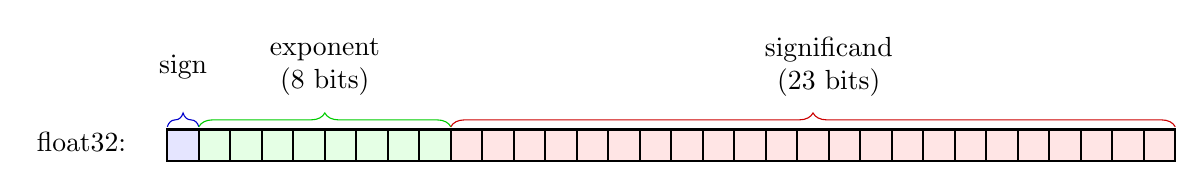
\begin{tikzpicture}[scale=.8]
    \node[anchor=south east] at (-.5, 0) {float32:};
    \draw[thick,fill=blue!10!white] (0, 0) rectangle ++ (.5, .5);
    \foreach \x in {1, ..., 8} {
      \draw[thick,fill=green!10!white] (\x/2, 0) rectangle ++ (.5, .5);
    }
    \foreach \x in {9, ..., 31} {
      \draw[thick,fill=red!10!white] (\x/2, 0) rectangle ++ (.5, .5);
    }
    \node at (0.25, 1.5) {sign};
    \node[align=center] at (2.5, 1.5) {exponent\\(8 bits)};
    \node[align=center] at (10.5, 1.5) {significand\\(23 bits)};
    
    \draw [blue!80!black,decorate,decoration = {brace, amplitude=5pt, raise=1pt}] (0,0.5) --  (.5,.5);
    \draw [green!80!black,decorate,decoration = {brace, amplitude=5pt, raise=1pt}] (.5,0.5) --  (4.5,.5);
    \draw [red!80!black,decorate,decoration = {brace, amplitude=5pt, raise=1pt}] (4.5,0.5) --  (16,.5);
  \end{tikzpicture}
  
  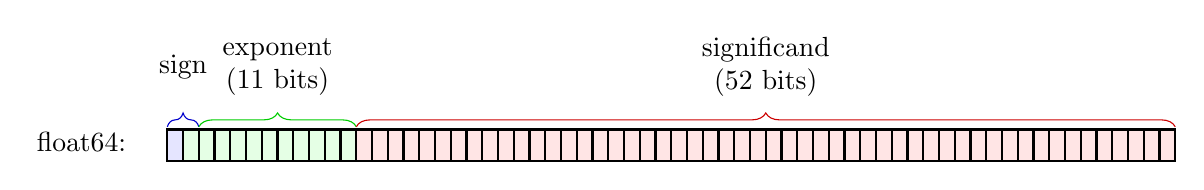
\begin{tikzpicture}[scale=.8]
    \node[anchor=south east] at (-.5, 0) {float64:};
    \draw[thick,fill=blue!10!white] (0, 0) rectangle ++ (.25, .5);
    \foreach \x in {1, ..., 11} {
      \draw[thick,fill=green!10!white] (\x/4, 0) rectangle ++ (.25, .5);
    }
    \foreach \x in {12, ..., 63} {
      \draw[thick,fill=red!10!white] (\x/4, 0) rectangle ++ (.25, .5);
    }
    \node at (0.25, 1.5) {sign};
    \node[align=center] at (1.75, 1.5) {exponent\\(11 bits)};
    \node[align=center] at (9.5, 1.5) {significand\\(52 bits)};
    
    \draw [blue!80!black,decorate,decoration = {brace, amplitude=5pt, raise=1pt}] (0,0.5) --  (.5,.5);
    \draw [green!80!black,decorate,decoration = {brace, amplitude=5pt, raise=1pt}] (.5,0.5) --  (3,.5);
    \draw [red!80!black,decorate,decoration = {brace, amplitude=5pt, raise=1pt}] (3,.5) --  (16,.5);
  \end{tikzpicture}
  % \includegraphics[width=.7\textwidth]{figs/computation/floating-point.pdf}
  \caption{Floating-point representation of numbers.}
  \label{fig:floating-point}
\end{figure}

\textbf{IEEE-754 Bit Layout}\quad We consider this briefly for concreteness' sake; the IEEE-754 standard is a very common format for representing floating-point numbers in computer hardware. For a floating-point number in this format, bits are divided into sign ($s$), exponent ($e$), and fraction/significand ($f$). For normal numbers (i.e., not zero, NaN, infinity, or subnormal),
\begin{equation*}
x = (-1)^s \times (1.f)_2 \times 2^{e-\text{bias}}
\end{equation*}
where the notation $(1.f)_2$ means the binary representation of the fraction $f$ with a leading 1 (implicit).In float32, $s=1$ bit, $e=8$ bits (bias $127$), and $f=23$ bits. In float64, $s=1$, $e=11$ bits (bias $1023$), and $f=52$ bits. The bit indices for float32 are $31$ (sign) $\mid$ $30\text{--}23$ (exponent) $\mid$ $22\text{--}0$ (fraction) (\autoref{fig:floating-point}). As an example (float32),
\begin{equation*}
\underbrace{0}_{s} \underbrace{01111100}_{e} \underbrace{01000000000000000000000}_{f}
\implies 
(-1)^0 \times (1.01)_2 \times 2^{-3} = 1 \times 1.25 \times \frac{1}{8}= 0.15625
\end{equation*}
Binary expansions of most real numbers are non-terminating and must be truncated, e.g.,
\[ \pi = 1.10010010000011111101101010\ldots \times 2^{1} \]
so the significand is truncated, introducing representation error.

\textbf{Precision and Hardware}\quad There is a practical tradeoff between accuracy and speed/memory. On most CPUs, double precision (float64) is the default and well optimized (e.g., MATLAB uses float64 by default). Many GPUs deliver highest throughput with float32 or even float16; low-precision arithmetic is common in machine learning. Choose the lowest precision that maintains the needed accuracy, and be mindful of mixed-precision casts when moving data between CPU and GPU. (In 10.34, this is not a significant consideration, but it is important to be aware of this fact.)

\textbf{Round-off and Machine Epsilon}\quad One specific type of numerical error arising from finite precision is round-off error. Every time an arithmetic operation is performed, the result must be rounded to the nearest representable number. Machine epsilon ($\epsilon_{\text{mach}}$) is an upper bound on the relative error due to rounding:
\begin{equation*}
    \epsilon_{\text{mach}} =
    \begin{cases}
        1.192\cdot 10^{-7} & \text{for float32} \\
        2.2204\cdot 10^{-16} & \text{for float64}
    \end{cases}
\end{equation*}
Simply put, $\epsilon_{\text{mach}}$ is the difference between 1 and the next largest floating point number for a given representation. For example, if we were to check the condition $1 + \epsilon_{\text{mach}}/2 \stackrel{?}{=} 1$ using single- or double-precision in some programming language, we would be told that indeed $1 + \epsilon_{\text{mach}}/2 = 1$, which is obviously not correct mathematically. However, adding anything larger than $\epsilon_{\text{mach}}$ to 1 will give the expected result.

% Rounding-off error is the primary drawback of finite precision. Even simple calculations can introduce numerical errors, so we must be careful when designing numerical algorithms. If we use MATLAB to calculate \verb|1 - 3 * (4 / 3 - 1)|, we get \verb|2.22e-16|, which is not zero (the analytical solution). However, if we use MATLAB to calculate \verb|1 - (3 / 3 * 4 - 3)|, we get \verb|0|. This shows that if we design numerical algorithms with care (in this case, that simply means applying the distributive property), we can avoid some of the pitfalls of finite precision. Finally, even though they seem small, the errors associated with floating-point arithmetic can compound and magnify in large calculations, leading to significant errors.

\textbf{Ordering Calculations}\quad Because floating-point numbers are only approximations, the way we arrange computations can create or avoid error. The most common manifestation of this is known as ``catastrophic cancellation'': subtracting nearly equal quantities wipes out correct digits and magnifies rounding noise. For example, the algebraically equivalent expressions $1-3(4/3-1)$ and $1-(3/3\cdot 4-3)$ can result in $2.22\times10^{-16}$ versus $0$ in double precision; this is because the first forces a small difference subtraction while the second avoids it. Similar issues show up when computing $1-\cos x$ for small $x$ (use the fact that $1-\cos x \approx 2\sin^2(x/2)$ at small $x$ to compute this instead), summing terms with very different magnitudes (sum smaller terms first or use compensated summation), or applying the quadratic formula when $b^2\gg4ac$ (use $2c/(-b\mp\sqrt{b^2-4ac})$ for the small root). The practical rule you should know for 10.34 is simple: choose algebraic forms that avoid subtracting nearly equal numbers, keep intermediate values on similar scales (rescale when helpful), and use numerically stable library routines (i.e., no need to reinvent the wheel if MATLAB has something you need). Otherwise, tiny rounding errors can accumulate over many operations into visible inaccuracies.

\textbf{Overflow and Underflow}\quad  Overflow/underflow describes the situation where numerical calculation exceeds the limits of floating-point formats. It occurs when we try to store numbers that are too large (overflow) or too small (underflow) for our chosen representation. The finite precision and finite exponent limit the range: approximately $10^{-38} \leq |x| \leq 10^{38}$ for float32 and approximately $10^{-308} \leq |x| \leq 10^{308}$ for float64. Thus, we may need to rescale our numbers to avoid overflow/underflow. Generally, though, this is not something we need to worry much about.

\begin{warningBox}
    \textbf{Warning: Intermediate Steps Can Overflow!}
    An expression can overflow during an intermediate step even if the final answer is perfectly representable.

    For example, calculating the hypotenuse $\sqrt{a^2 + b^2}$ with $a=10^{200}$ and $b=10^{200}$ will fail because $a^2$ overflows. A robust function like MATLAB's \texttt{hypot(A, B)} avoids this by rescaling first.
\end{warningBox}

\textbf{Truncation Error and Convergence}\quad Even with infinite precision, numerical errors arise due to the approximate nature of many algorithms. Iterative methods and series expansions approximate mathematical functions, introducing errors that depend on the number of terms or iterations used. To illustrate this, let's compare two different algorithms for approximating the same mathematical constant: \(\pi\). The Leibniz series is a simple infinite series that approximates \(\pi\) as
\begin{equation*}
\pi = 4 \sum_{n=0}^\infty \frac{(-1)^n}{2n+1}
\end{equation*}
This series converges very slowly. To achieve just two decimal places of accuracy, we need to sum over several hundred terms. The slow convergence means more iterations are required for high precision, increasing computational effort and the potential for cumulative numerical errors. In contrast, we can consider one of Ramanujan's series for \(\pi\), which converges extremely rapidly:
\begin{equation*}
    \frac{1}{\pi} = \frac{2\sqrt{2}}{9801} \sum_{n=0}^\infty \frac{(4n)! (1103 + 26390n)}{(n!)^4 396^{4n}}
\end{equation*}
This series is remarkable because each term adds approximately eight additional correct decimal places to the approximation of \(\pi\). Therefore, summing just a few terms yields a highly accurate value. The convergence of these two series to the true value of $\pi$ is shown in \autoref{fig:pi-approximation}. The Ramanujan series converges to within machine epsilon after just 3 terms!

\begin{figure}[!h]
    \centering
    \includegraphics[width=.65\textwidth]{figs/computation/pi-convergence.pdf}
    \caption{Convergence of two series approximating \(\pi\). Machine epsilon is approximately \(2.22 \cdot 10^{-16}\) here, so values within this range are essentially as converged as numerically possible.}
    \label{fig:pi-approximation}
\end{figure}

\subsection{Computational Complexity}
As suggested earlier when discussing numerical error, we need to understand not just how to solve a problem, but also how efficiently it can be solved as the problem size increases. This efficiency is quantified using the concept of \textbf{computational complexity}. Specifically, we focus on \textbf{time complexity}, which measures the number of elementary operations an algorithm requires relative to the size of its input (the size of the input is typically denoted by $N$).

To express computational complexity, we generally use \textbf{big-O notation}. This mathematical notation describes an upper bound on the growth rate of a function so that we can focus on the most significant factors that affect an algorithm's performance as the input size becomes large. Mathematically, we say that a function $f(N)$ is $O(g(N))$ if there exist positive constants $c$ and $N_0$ such that
\begin{equation*}
    \left|f(N)\right| \leq c \cdot \left|g(N)\right| \quad \text{for all } N \geq N_0
\end{equation*}
This definition means that for sufficiently large values of $N$, the function $f(N)$ does not grow faster than a constant multiple of $g(N)$. Again, we stress that big-O notation captures the dominant term of $f(N)$ as $N$ approaches infinity, ignoring lower-order terms and constant factors that become insignificant at large scales.

\begin{exampleBox}
    \textbf{Example}: We consider two algorithms designed to solve the same problem with input size $N$. Algorithm A has a time complexity of $f_A(N) = 5N^2 + 10000$. Algorithm B has a time complexity of $f_B(N) = 2N^3 + N$. We can express the time complexity of each algorithm using big-O notation:
    \begin{align*}
        f_A(N) &= O(N^2) \\
        f_B(N) &= O(N^3)
    \end{align*}
    To see the practical impact, let's compare the number of operations required as $N$ increases:
    \begin{center}
        \begin{tabular}{c|c|c}
            \textbf{Problem Size ($\boldsymbol{N}$)} & \textbf{Operations in Algorithm A} & \textbf{Operations in Algorithm B} \\
            \hline
            $10$ & $1.05\cdot 10^4$ & $2.01\cdot 10^3$ \\
            $100$ & $6\cdot 10^4$ & $2.0001\cdot 10^6$ \\
            $1000$ & $5.01\cdot 10^6$ & $2.000001\cdot 10^9$ \\
            $10000$ & $5.000001\cdot 10^{10}$ & $2.0000000001\cdot 10^{15}$ \\
        \end{tabular}
    \end{center}
    As the table shows, Algorithm B requires significantly more operations than Algorithm A as $N$ grows (but notice this is NOT true at small $N$!), making it less practical for large problem sizes. This also follows directly from the big O notation, which tells us that $f_B(N)$ grows faster than $f_A(N)$.

    To be even more concrete, let's assume that each operation takes $10^{-8}$ seconds, which is reasonable for a modern CPU. Then, we can construct the table below:
    \begin{center}
        \begin{tabular}{c|c|c}
            \textbf{Problem Size ($\boldsymbol{N}$)} & \textbf{Algorithm A Runtime} & \textbf{Algorithm B Runtime} \\
            \hline
            $10$ & $0.105 \,\text{ms}$ & $0.0201 \,\text{ms}$ \\
            $100$ & $0.6 \,\text{ms}$ & $20.001 \,\text{ms}$ \\
            $1000$ & $50.1 \,\text{ms}$ & $20 \,\text{s}$ \\
            $10000$ & $8.33 \,\text{min}$ & $231 \,\text{days}$ \\
        \end{tabular}
    \end{center}
\end{exampleBox}

The above example shows how algorithms with lower computational complexity dramatically reduce computation time, especially for large $N$. The difference between $O(N^3)$ and $O(N^2)$ algorithms (and more generally, any two algorithms with different associated time complexities) can be the difference between a project being feasible or not.

Finally, we briefly mention the concept of \textbf{space complexity}, which measures the amount of memory an algorithm requires relative to the size of its input. Space complexity is also expressed using big O notation, but we will not discuss it further in this course. However, it is important to remember that memory usage can be just as important as time complexity, especially when working with large datasets or on memory-constrained devices.

%%% Local Variables:
%%% mode: LaTeX
%%% TeX-master: "../main"
%%% End:
